\section{Experiment Execution}\label{sec:execution}

\textbf{Hardware.} A single S2-group workstation hosts the measured stack. The machine provides \textbf{two RTX 4000 Ada cards (20\,GB each)}; GPU~0 runs the inner CNN training and GPU~1 serves the proposer at int4. Idle draw was recorded in experiment notes as 8.63\,W (GPU~0) and 7.90\,W (GPU~1), but the underlying idle traces were not preserved. No idle subtraction is therefore applied: all reported energies are gross over the session boundary and include standby and weight-residency draw. Separate GPUs remove co-location contention and provide direct board-level readings, but whole-session GPU~0/GPU~1 totals are device-associated quantities rather than pure training/proposer phase energy. The CPU-served proposer phase remains pending and is not described as executed.

\textbf{Software infrastructure.} The S2 \texttt{experiment-runner} framework \cite{karsten2025experimentrunner} acts as the \emph{session-level orchestrator}: each run in its run table is one complete \texttt{autoresearch} session. Per run, the runner instantiates the program, selects a proposer endpoint, launches the agent session, and starts two profilers at approximately 10\,Hz: a dedicated NVML sampler for both GPUs and \texttt{EnergiBridge} \cite{sallou2023energibridge} for the host. On this AMD machine the archived EnergiBridge schema exposes one \texttt{CPU\_ENERGY (J)} package counter and no separate DRAM counter. The original parser looked only for Intel-style \texttt{PACKAGE\_ENERGY}/\texttt{DRAM\_ENERGY} columns, leaving \texttt{E\_cpu\_J} blank; CPU-package energy is nevertheless recoverable from the raw trace by differencing the counter over the same session timestamps used for NVML. The registered inferential pipeline therefore remains GPU-only, with measured GPU+CPU-package totals reported as a post-hoc sensitivity analysis. \textbf{Deviation:} the upstream \texttt{autoresearch} repository publishes the protocol and its inner workload but contains no agent loop, so its fixed-budget keep/revert protocol was re-implemented, with patience and loop budget enforced in code. Each Phase-1 archive contains the session log, both raw traces, summary, harness log, and recipe-history bundle. The training-file content record is \texttt{eb632882}; session logs separately record harness repository SHA \texttt{7065bf27}; these identify different artifacts and are not presented as one commit. The two proposer builds are pinned to their HuggingFace revisions (\texttt{Qwen/Qwen3-14B-AWQ} at \texttt{31c69ef}, \texttt{QuixiAI/Qwen3-30B-A3B-AWQ} at \texttt{1ba5586}).

\textbf{Why a purpose-built agent loop.} The upstream \texttt{autoresearch}
repository publishes the protocol and its default inner workload but does not
ship a runnable agent loop, so some implementation was unavoidable. The more
substantive question is why a general-purpose agent framework (Aider, OpenHands,
SWE-agent, AutoGen) was not used instead, since any of them can edit a file in a
loop. Four requirements of this experiment are incompatible with how such
frameworks are built.

\emph{Factors must be enforced, not requested.} Patience and loop budget are
independent variables, so they must mean exactly the same thing for both
proposers. A framework expresses such policy in the prompt and relies on the
model to comply; compliance varies by model, which would confound the factor with
the arm under test. Here both are enforced in Python, so \texttt{patience}~$=3$ is
identical for dense and MoE by construction.

\emph{Iteration attribution needs sharp phase boundaries.} The analysis attributes
iteration-level GPU energy to proposing and training by cutting the 10\,Hz traces
at the instant proposing stops and training starts. The loop
emits \texttt{propose\_start/end} and \texttt{train\_start/end} with paired
wall-clock and monotonic timestamps for exactly this purpose. General agents
interleave tool calls, streaming and internal retries, and expose no such
instant; without it, the decomposition would revert to a modelled estimate, which
is the threat this design exists to avoid.

\emph{Infrastructure failure must be separable from agent failure.} Frameworks
retry internally and absorb the distinction. This experiment depends on it: a
flaky endpoint would otherwise be indistinguishable from a poor proposer. The
taxonomy is what allows a session with a 0\,\% infrastructure-error rate and a
30\,\% agent-error rate to be reported as valid evidence, with the latter treated
as data rather than as noise.

\emph{Every proposer attempt must be accounted.} Tokens, latency, outcome and
finish reason are recorded per attempt, under a time budget spanning retries.
Hidden retries would make proposer energy uninterpretable, since a single
iteration could contain an unknown number of inferences.

This is not a from-scratch system. Orchestration is \texttt{experiment-runner},
energy measurement is \texttt{EnergiBridge}, serving is vLLM \cite{kwon2023vllm}, and the protocol is
Karpathy's; the custom component is only the loop, the one place where
general-purpose design conflicts with measurement requirements. The cost is
recorded in Section~\ref{sec:threats}: the results are conditional on this
harness, and the harness demonstrably shapes them, so it is pinned, unit-tested
and shipped in the replication package rather than treated as a neutral conduit.

\begin{figure}[htbp]
\centering
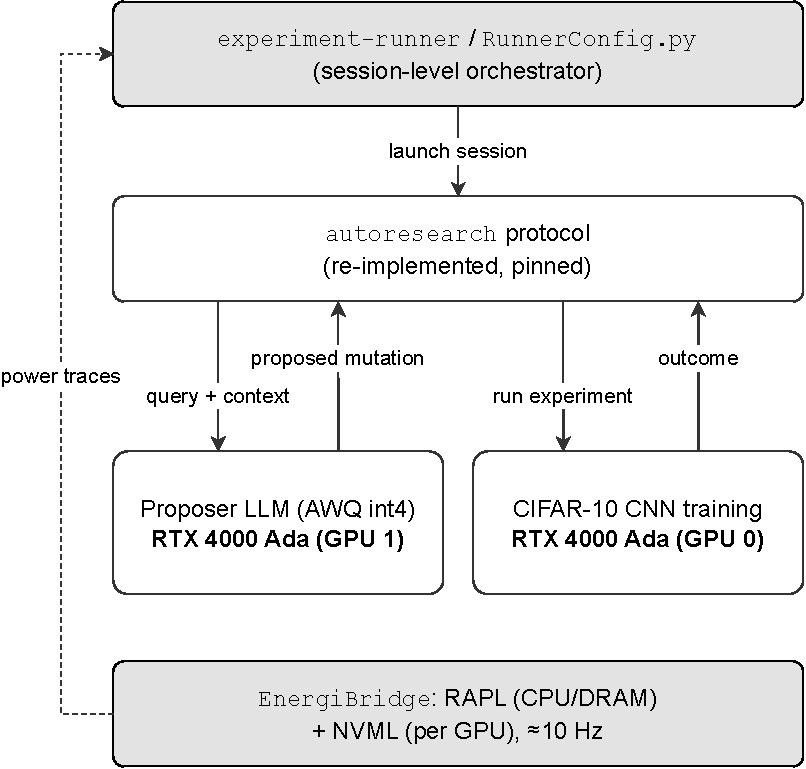
\includegraphics[width=\columnwidth]{figures/infra.drawio.pdf}
\caption{Measurement infrastructure: session-level orchestration over the agent loop, with per-GPU board measurement and phase-aligned iteration attribution.}
\Description{Architecture diagram showing experiment-runner launching the agent loop, which exchanges proposals with a Qwen model on GPU 1 and runs CIFAR-10 training on GPU 0, while EnergiBridge and NVML record energy traces.}
\label{fig:infra}
\end{figure}

\textbf{Executed procedure.} Calibration set the inner training budget to 45\,s: the reference recipe left $+15.27$\,pp of headroom above baseline, compared with $+14.32$\,pp at 240\,s, while signal-to-noise differed by only 8\,\%. Eight baseline repeats with a 120\,s cool-down gave a detrended standard deviation of 0.62\,pp, from which the keep threshold $\epsilon=0.0123$ was derived. The 24-session Phase-1 factorial then ran with randomized, interleaved cells; the completed reasoning and temperature follow-ups added 30 sessions. All 54 campaign sessions are valid. The planned eight-session CPU-served proposer subset was not launched while supervisor feedback is pending. The recorded GPU idle rates are retained only as contextual observations because their raw traces and a CPU-idle measurement are unavailable; they do not enter a correction.
